\newpage
\section{Fundamentals}
\label{sec:fundamentals}

A basic description of what a \ac{PUF} is and how it works has been given in section \ref{sec:motivation}.
In order to conceptualize an authentication infrastructure around \acp{PUF},
a deeper understanding of how \acp{PUF} work, what types or classes of them exist and
how they relate to their environment in terms of inputs and outputs, is needed.

\subsection{Definitions and Basic Concepts}
\label{sec:puf_def_of_terms}

In this section, important terms needed for describing PUFs are explained.
Then, the term \acf{PUF} itself and some additional characteristics are defined.

\acp{PUF} can be physically constructed in different ways.
All PUFs constructed using the same structural design, belong
to the same PUF \emph{class} $P$. \cite[][p. 14]{Maes2013}

One specific device manufactured according to the design of a PUF class is called
an \emph{instance} of the class. Each time a new device is manufactured, a new PUF is \emph{instantiated}.
The process of creating a new instance of a class is also called the creation procedure $P.Create$, which
returns a new instance $puf$.
Each instance has a certain state. This state is usually determined during construction of the PUF, but
certain classes of PUFs can also have configurable state.
This type of state can be modified even after instantiation using some form of external input $x$.
This input is called \emph{challenge} and is applied to the instance, altering its state.
A PUF with state that is configured using challenge $x$ is called $puf(x)$. \cite[][p. 14]{Maes2013}

Each PUF instance has an evaluation procedure called $puf.Eval$ or, if the particular instance has configurable state,
$puf(x).Eval$.
As \acp{PUF} are physical objects, the evaluation procedure is some kind of physical experiment resulting in a measurement,
which depends on the internal state of the instance.
This measurement is the result of $puf.Eval$ and also called the PUF's \emph{response} \cite[][p. 14f]{Maes2013}.
The set consisting of a challenge and its corresponding response is called a \ac{CRP}.

Many different definitions of the term \emph{PUF} exist in the literature \cite{Ruehrmair2010} \cite{Guajardo} \cite{Maes2013}.
\citeauthor*{Pappu2002} first defined the concept now known as PUF as a "Physical One-Way Function",
making them the physical equivalent of the mathematical concept of a one-way function. \cite{Pappu2002}

To summarize the concept of a PUF concisely, \citeauthor*{Maes2013} defines \acp{PUF} in the following way:

"A PUF is an expression of an inherent and unclonable instance-specific feature of a physical object” \cite[][p. 12]{Maes2013}

To explain this definition further, he compares it to a human fingerprint, as it is similar in many regards.
Fingerprints can not just be used to confirm that someone is actually a human,
but are a feature which can be used to identify a specific individual, just like
a \ac{PUF} can be used to identify a specific instance of a class of \acp{PUF}.
Therefore PUFs are instance-specific. \cite[][p. 11f]{Maes2013}

Fingerprints are inherent, in that humans are born with them.
PUFs are also inherent, because they are a direct result of an object's creation process.
Theoretically, every physical object has some kind of property which fits the definition of a PUF,
as no two objects are exactly identical. Whether or not these properties are useful or not,
depends on their intra- and inter-distance and how easily they can be measured. \cite[][p. 12]{Maes2013}

Lastly, fingerprints are unclonable, as there is no way to create a human clone with exactly the same fingerprint.
This is also a central requirement for an object's property or feature to be considered a PUF .\cite[][p. 12]{Maes2013}

In addition to \citeauthor{Maes2013}, the definition given by \citeauthor*{Guajardo} in \cite{Guajardo} should be mentioned,
as it was one of the first attempts at a formalized definition of the term PUF \cite[][p. 84f]{Ruehrmair2010}.
This definition matches \citeauthor{Maes2013}' definition very well, in that it also focuses on the inherency of PUFs stemming
from uncontrollable random variations in the manufacturing process.
Furthermore, he defines a PUF as a function, which maps a challenge to a response .\cite[][p. 65f]{Guajardo}

Additionally, multiple assumptions about PUFs are made:
\begin{itemize}
    \item A response $R_i$ received from a PUF instance based on challenge $C_i$, should not give significant
          information about another response $R_j$ resulting from challenge $C_j$.
          This means, that by knowing one \ac{CRP} of a PUF instance, no conclusions about other \acp{CRP}
          should be possible.
    \item Without access to the PUF, one should not be able to work out the correct response $R_i$ to a challenge
          $C_i$, except for randomly guessing it.
    \item He also assumes, that PUFs are "tamper evident". This means, that the process of
          collecting detailed information about a specific PUF instance to the point of being able to predict \acp{CRP} should
          alter the instances behavior, essentially destroying it.
\end{itemize}

In a recent review article \cite{McGrath2019}, \citeauthor*{McGrath2019} extend the definitions mentioned previously
with some additional properties:
\begin{itemize}
    \item \emph{Robustness}: PUFs need to be stable over time. This means, that their behavior doesn't change with
          increasing age and \acp{CRP} stay consistent
    \item \emph{Hard to replicate}: Creating a physical copy of a PUF instance needs to be difficult in order to
          preserve the uniqueness and instance-specificity of PUFs.
          Replicating a PUF would allow an attacker to gain access to a system which employs PUF-based security.
    \item \emph{Unpredictable}: Predicting how an instance would respond to a given challenge needs to be hard or impossible.
          This ensures that an attacker would not be able to create a model of an instance which would again
          allow them to gain access.
\end{itemize}

For many PUF classes, external physical conditions influence the result of the evaluation procedure.
Such conditions could be temperature or voltage level.
Using the example of a PUF which is influenced by the environment temperature, an evaluation with
$T_{env} = 80^{\circ}C$ would be written as $puf(x).Eval^\alpha$ with $\alpha = T_{env}$. \cite[][p. 15]{Maes2013}

The usability of a PUF class greatly depends on the behavior of the responses given the same or different instances,
challenges and conditions.

% Could elaborate on the term PUF, see Maes p.20ff

% \cite{Maes2013} % Properties

% \cite{Katzenbeisser2012} % Security Properties

\subsection{Statistical Consideration of PUFs}
\label{sec:statistical_considerations}

As PUFs use internal random variations for generating responses, the challenge-response behavior is never completely
consistent and always contains variability. For PUFs to be useful for authentication or other use-cases,
these variations need to be considered. The statistical knowledge required is presented in this section.

\subsubsection{Hamming Distance}

After post processing, PUF responses typically consist of bit vectors. A bit vector $Y$ has length $|Y|$.
The \emph{Hamming Distance} is a measure which quantifies the distance between two bit vectors of the same length.
It is typically used in error correction for measuring the amount of flipped bits in a transmission.
Specifically, it is the number of bits with differing values in both vectors. It is denoted as $HD(Y;Y')$, where
$Y$ and $Y'$ are two bit vectors of the same length. \cite[][p. 173f]{Maes2013}

The \emph{Fractional Hamming Distance} is the number of bits with differing values divided by $|Y|$. \cite[][p. 173f]{Maes2013}

As an example we define two bit vectors:
\[Y =  01110111\]
\[Y' = 01101011\]

In this example the length of the bit vector is $8$ and $3$ bits are different between the two.
The Hamming Distance and Fractional Hamming Distance are calculated like this:
\[HD(Y;Y') = 3\]
\[FHD(Y;Y') = \frac{HD(Y;Y')}{|Y|} = \frac{3}{8} = 0.375\]

\subsubsection{Intra- and Inter-Distance}
\label{sec:intra_inter_distance}

The \emph{intra-distance} of two PUF responses describes the distance between two responses from the same PUF
instance given the same challenge. It is important to understand how the intra-distance behaves for a given class,
in order to make assumptions about how reproducible the results for a given instance are \cite[][p. 16f]{Maes2013}.
Although any distance metric could be used for quantifying this distance, almost all of the literature considered
in this thesis uses the Hamming distance.

External conditions can have a big impact on the typical intra-distance of a class.
Typically, two responses generated at different external conditions have a larger intra-distance,
than those generated under the same conditions.
One has to understand which external conditions influence responses in which way.
Often, a reference value $\alpha_{ref}$ for the condition is set before evaluating the responses for
varying values experimentally.
It is important to understand the worst case intra-distance of a given instance.
This is done by defining a range of conditions and measuring responses at both ends of the spectrum.
\cite[][p. 16f]{Maes2013}


The \emph{inter-distance} describes the distance between two responses from different PUF instances
using the same challenge.
A high inter-distance means that it is easier to distinguish two unique instances of a given class
and correctly identify them. \cite[][p. 18ff]{Maes2013}

\subsubsection{Central Statistical Properties}
\label{sec:central_statistical_properties}

For a class of PUF to be statistically relevant for security related purposes, it has to have two central
statistical properties.

\textbf{Uniqueness}

A PUF class has the property of uniqueness, if there is a high probability, that the inter-distance between two given instances
is large. If this probability was relatively small, there would be a high chance, that two instances have a similar
challenge-response behavior and would thus not be considered unique. \cite[][p. 53]{Maes2013}

\textbf{Identifiability}

For instances of a class to be generally identifiable, responses need to be reproducible and instances have
to be unique. This ensures that it is more likely for responses from the same instance to be similar,
than for responses from two different instances.
This means that the probability of the inter-distance being larger
than the intra-distance of the PUF needs to be high. \cite[][p. 53f]{Maes2013}

More information about inter- and intra-distance, and the statistical properties of PUF is given in section \ref{sec:puf_authentication}.

\subsection{Classification of PUFs}
\label{sec:classification}
% TODO: more sources
%\cite{Gao2020}  Taxonomy
%\cite{Herder2014} Types
%\cite{McGrath2019} % Taxonomy

PUF constructions can be classified in different ways \cite[][p. 4ff]{McGrath2019}.
In this section PUFs are classified by their specific properties, as opposed to using
e.g. chronological classification.

\subsubsection{Electronic vs. Non-Electronic PUFs}

Firstly, PUFs can be classified by their electronic characteristics. \cite[][p. 22]{Maes2013}

% Could incorporate examples for each class from different sources

\emph{Non-electronic PUFs} are based on technologies or materials which are not based on electronics.
This could be the random molecular structure of an object causing light to be scattered in different ways or surfaces
to have different characteristics.
The non-electronic nature of this class is limited to the random variation itself.
Evaluation, including the measurement, post-processing and digitization of a response, can be done electronically \cite[][p. 22]{Maes2013}.
PUFs using this form of electronic evaluation of a non-electronic property are also called \emph{Hybrid PUFs} \cite[][p.]{McGrath2019}.
This is the most common form of non-electric PUFs, as responses typically need to be compared to database entries,
which is not practical without electronic data processing.

\emph{Electronic PUFs} are the counterpart to non-electronic PUFs.
They rely on constructions which have electronic characteristics that can be used as PUFs.
This could be resistance, capacitance or others.
Responses are commonly evaluated using electronic means.
Usually electronic variations in these PUFs occur due to non-electronic physical characteristics, such as the
length of a wire.
There are PUF constructions which can't be strictly classified as either electronic or non-electronic,
as they combine electrical elements with properties of non-electronic materials to introduce randomness.
\cite[][p.22f]{Maes2013}

\emph{Silicon PUFs} are a subclass of electronic PUFs consisting of integrated electronic circuits
embedded on a silicon chip \cite[][p. 23]{Maes2013}.
Silicon PUFs have the advantage of being contained within the circuit of a chip, which can be directly embedded
into an electronic circuit board and interact as part of an embedded system or computer.
They can thus be used as cryptographic elements in security systems. \cite[][p. 23]{Maes2013}

\subsubsection{Implicit vs. Explicit Random Variations}

A classification by implicitness is also sensible.
PUFs need some kind of physical property which introduces randomness that makes
an instance unique and ensures, that a response can not easily be inferred from a given challenge.
Implicitness depends on wether the manufacturing process needs to be specifically adapted by the manufacturer in order
to introduce randomness into the object, or if the randomness is inherently present in all objects,
without changing the process.
The latter would be called an \emph{implicit random variation}, while randomness introduced by adjusting the
process (e.g. adding additional components) is called an \emph{explicit random variation}. \cite[][p. 24]{Maes2013} \cite[][p. 3]{McGrath2019}

A meaningful benefit to implicit random features exists from a security standpoint.
As even manufacturers are not able to control these variations, there is no entity that has to
be trusted, as nobody has the ability to remove or control the randomness of the given feature used for PUF evaluation.
In contrast, when using a PUF with explicitly introduced random variations, a level of trust towards the manufacturer
is required. If the manufacturer were to decide to intentionally manipulate PUF instances and introduce
equivalent behavior into several instances, the instance-specificity and unclonability principles of the PUF construction would be violated,
which has severe security implications \cite[][p. 24]{Maes2013} \cite[][p. 3]{McGrath2019}.
Additionally, implicit random variations reduce cost, as no extra steps are needed in manufacturing. \cite[][p. 3]{McGrath2019}

\subsubsection{Intrinsic vs. Extrinsic PUFs}

A PUF has an internal evaluation, if the evaluation function, which is the measurement of the random feature
and creation of a response, happens entirely within the PUF device itself, without requiring external
measurement equipment or analysis \cite[][p. 23f]{Maes2013}.
For a PUF to be considered an \emph{intrinsic} PUF, the random variation has to be implicit and the evaluation has to be internal.
If one of these criteria is not met, the class is classified as a non-intrinsic or \emph{extrinsic} PUF. \cite[][p. 3]{McGrath2019}

There are multiple advantages to internal evaluation.
If the measurement is taken as part of the PUF construction, there is no variation that can be introduced
by varying measurement equipment or execution, leading to more accurate results and less errors.
It is also more practical, as no specific equipment is needed to read responses.
Lastly there is a security advantage. While a response is kept within an instance and not exposed to the outside,
it can be considered secret and is not subject to attacks.
This would also be a benefit for an authentication system, as this secret could
then be used as part of cryptographic evaluations .\cite[][p. 23f]{Maes2013} \cite[][p. 3]{McGrath2019}

\citeauthor{Maes2013} describes an advantage of external evaluation procedures to be, that they allow better verification of a successful measurement.
As there is no way to inspect an internal evaluation, one has to trust that the PUF evaluation function is working as intended \cite[][p. 24]{Maes2013}.
On the other hand, according to \citeauthor*{McGrath2019} in \cite{McGrath2019}, internal evaluation is more accurate.

% TODO: more detail

% Examples for non-intrinsic PUFS see Maes2013 p.24f

\subsubsection{Strong vs. Weak PUFs}
\label{sec:strong_weak_pufs}

This classification is based on the number of \acp{CRP} that a single PUF instance has \cite[][p. 2]{McGrath2019},
which correlates with how secure the challenge-response behavior of that PUF class is \cite[][p.25]{Maes2013}.
Imagine an attacker having an extended period of time with access to a specific PUF instance.
They would certainly use that time to try and find out all possible \acp{CRP} of the instance, as this
would give them unlimited access to whatever system the PUF is used to protect. \cite[][p.25]{Maes2013}

Strong PUFs have the property, that after this time, there would still be a high probability of finding a challenge,
to which the attacker does not know the response.
This implies, that the number of \acp{CRP} must be large enough, to make brute forcing all possible solutions impossible
within the given time.
It also implies, that the instance must be entirely unpredictable. Otherwise it would be possible to create a model or
simulation of the PUF instance, which would behave exactly like the real instance and be able to
deliver the correct response to every given challenge \cite[][p.25]{Maes2013} \cite[][p. 66]{Guajardo}.
An additional characteristic of a strong PUF is, that the number of \acp{CRP} scales exponentially with the physical devices size.
This means, that by increasing the size, of a PUF can be made much more secure \cite[][p. 2]{McGrath2019}.

The properties of strong PUFs have interesting implications for authentication systems.
In a system based on symmetric cryptographic keys or \ac{PKI}, the secret used for authentication is useless
if a third-party had access to the (private) key at some point in the past. % Some source here would be nice ig...
In contrast, if strong PUFs are used for encryption, there is no way for an attacker to falsely authenticate,
as long as the attacker doesn't have physical access to the device at the time of authentication \cite[][p. 2]{McGrath2019}.
The large set of \acp{CRP} also makes authentication using strong PUFs resistant to eavesdropping, because
no challenge ever has to be used twice. This means, that even if an attacker gets hold of a \ac{CRP}, they
are not able to compromise future authentications, as a different challenge would be given every time.

Weak PUFs have a relatively small set of \acp{CRP}, which means that an attacker
could brute-force or record all possible \acp{CRP} in a reasonable amount of time \cite[][p. 2]{McGrath2019}.
Weak PUFs could also be predictable enough to be modelled \cite[][p.25]{Maes2013} \cite[][p. 66]{Guajardo} and
the number of \acp{CRP} doesn't typically scale with device size \cite[][p. 2]{McGrath2019}.
An additional characteristic is, that the size of the set of \acp{CRP} does generally not scale exponentially,
but linearly or in a polynomial order, when increasing device size \cite[][p. 2]{McGrath2019}.
This limits the practical applications of weak PUFs. If they were used in an authentication system,
an attacker could easily breach security because of the downsides mentioned.
A benefit of weak PUFs and the reason for them being preferred for some applications is,
that they are typically much easier and cheaper to manufacture. \cite[][p.25]{Maes2013}

\subsection{Popular PUF Implementations}
\label{sec:puf_implementations}
Many different concepts for PUF constructions have been explored in the literature.
While some, like the Arbiter PUF, are well established and have been widely researched,
others, like the MEMS PUF \cite{Aysu2013}, provide a more niche approach \cite[][p. 2]{McGrath2019}.
In this section, some of the most popular PUF constructions according to \cite{McGrath2019}
from different families are examined to get a sense of how they work internally,
what kinds of challenges they take, and what kinds of responses they emit.

\subsubsection{Arbiter PUF}

According to \cite[][p. 6]{McGrath2019}, this PUF concept was first proposed by \citeauthor*{Lee} in 2004 \cite{Lee}.
Arbiter PUFs use statistical variations in the time delay characteristics of electrical components like wires or transistors
in integrated circuits as a unique characteristic. \cite[][p. 176]{Lee}

A delay line makes it possible to introduce and control a time delay into an electrical signal.
These delays are usually in the range of nanoseconds to microseconds \cite[][p. 1]{Shahoei2014}.
In an arbiter PUF, two electrical signals are simultaneously emitted and
sent through two separate delay lines, which consist of a number of switch components
and terminate in a latch component.
Figure \ref{fig:arbiter_puf_circuit} shows the structure of an Arbiter PUF circuit.

\begin{figure}[H]
    \centering
    \caption{Structure of an Arbiter PUF}
    \label{fig:arbiter_puf_circuit}
    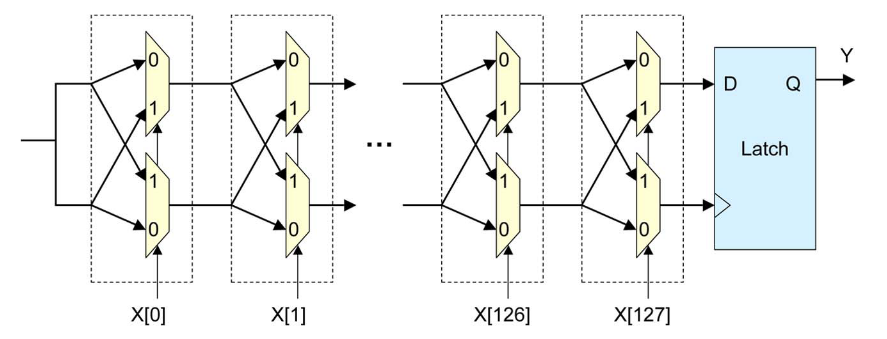
\includegraphics[width=1.0\textwidth]{arbiter_puf_circuit.png}
    \\
    Source: \cite[][p. 1130]{Herder2014}
\end{figure}

The challenge consists of $n$ bits, where $n$ is the number of switch components
in the delay line. In figure \ref{fig:arbiter_puf_circuit}, $n$ equals $128$.
Each bit configures the corresponding switch to adjust the delay path accordingly.
If a switch is set to $0$, the signals stay on their current paths,
if it is $1$, the signals cross.
At the end of the line, the latch component measures, which of the two signals arrives first.
If the paths are always symmetric regardless of switch position, a response of $0$ or $1$ is
equally likely. This would be ideal, as the variation in speed would only occur based on
variations in the manufacturing of the conductor and switches.
In practice, constructions can't always achieve exact symmetry because of space constraints. \cite[][p. 177]{Lee}

The delay of electrical components is dependant on external factors, namely
temperature, ambient noise levels and voltage variations.
The arbiter PUF solves this by not using absolute delay values, but relying on relative comparisons
between different delay characteristics. \cite[][p. 176]{Lee}

Arbiter PUFs belong to the group of fully electronic PUFs. The source of randomness is implicit, because it relies
on variations within the electrical components of the circuit, which can't be controlled in any way.
They also have internal response evaluation, which makes them intrinsic, and have a large set of \acp{CRP}
that increases exponentially while adding more switch components, making them strong PUFs. \cite[][p. 176]{Lee}


\subsubsection{SRAM PUF}

According to \cite[][p. 6]{McGrath2019}, this PUF concept was first proposed by \citeauthor*{Guajardo} in 2007 \cite{Guajardo}.
Compared to \ac{DRAM}, which is typically used as the main memory in modern computers, \ac{SRAM}
has higher power consumption and very complex internal circuitry, which makes it larger and more expensive.
However, it is still an important part in modern computers, as it allows for much lower access times than \ac{DRAM},
which makes it viable as a fast caching layer in the memory hierarchy \cite[][p. 2f]{Singh2013}.
An SRAM cache consists of peripheral circuitry which handles data input and output and address decoding.
They also consist of many SRAM cells, typically consisting of six transistors.
Each cell can hold one bit of information \cite[][p. 5]{Singh2013}.
The architecture of a typical bit cell is shown in figure \ref{fig:sram_puf_circuit}.
It consists of four load transistors $M_1 - M_4$, which store the information, two access transistors $M_5$ and $M_6$, a word line
$WL$ and the data bit-lines $BL$ and $\overline{BL}$, which carry data to and from the cell \cite[][p. 73]{Guajardo}.

The load transistors are connected in such a way, that they create a positive feedback loop.
If the voltage at node $Q$ tends towards being high, the feedback loop will amplify this tendency
and force the voltage to high. $Q$ and $\overline{Q}$ always have opposite states.
The voltage at node $Q$ dictates the bit of information stored within the cell. If $Q$ is high, the cell is $1$,
if it's low, the cell is $0$. \cite[][p. 31]{Singh2013}

\begin{figure}[H]
    \centering
    \caption{Circuit Diagram of SRAM PUF}
    \label{fig:sram_puf_circuit}
    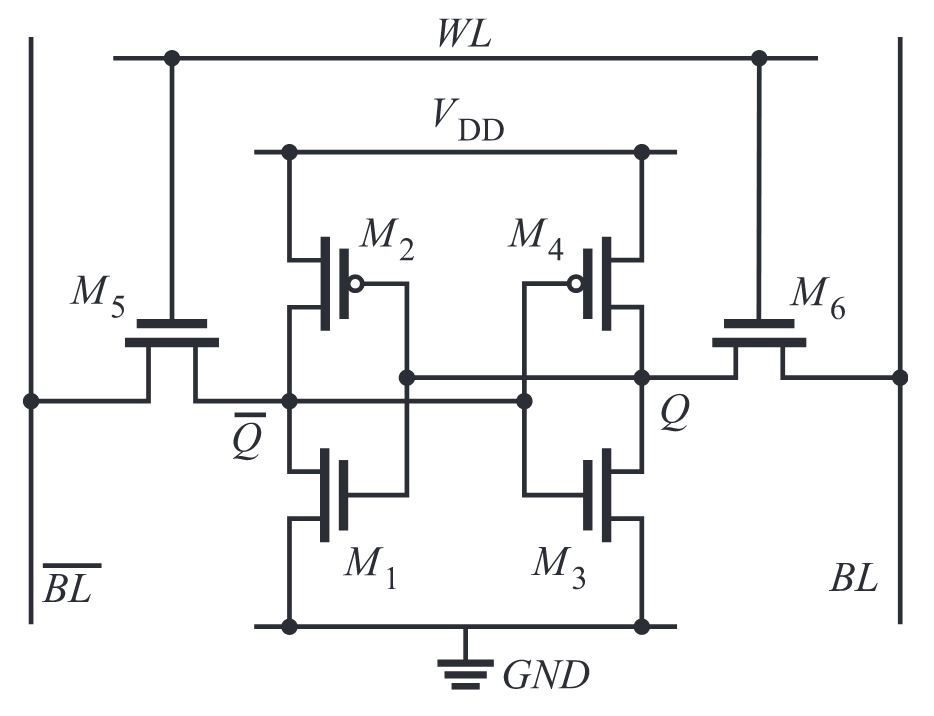
\includegraphics[width=0.6\textwidth]{sram_puf_diagram.png}
    \\
    Source: \cite[][p. 12]{McGrath2019}
\end{figure}

An SRAM cell can have three possible states:

\begin{itemize}
    \item \emph{Standby}: Here the word-line $WL$ is low, which disconnects the load transistors from the
          bit line. This means, that their state will not change as long as the load transistors are powered. \cite[][p. 31]{Singh2013}
    \item \emph{Reading}: Here, both bit-lines are set high. Then the access transistors are engaged,
          which connects the bit-lines to the load transistors. If the cell's state is $1$, $\overline{BL}$ will
          drop in voltage. If the state is $0$, $BL$ will drop in voltage. A sense amplifier measures, which of
          the bit-lines had a voltage drop and has thus read the cell.
          In the end, the word-line is set high again, to disconnect the cell \cite[][p. 32]{Singh2013}.
    \item \emph{Writing}: If a $1$ should be written, first $BL$ is set to $1$ and $\overline{BL}$ is set to $0$.
          $WL$ is set high to connect the cell to the bit-lines. Because the load transistors are much weaker
          than the bit-line drivers, they take the value of $BL$. The word-line is then disengaged\cite[][p. 36]{Singh2013}.
\end{itemize}

As SRAM cells have been scaled down to increase speed and size,
electrical deviations on an atomic-level become a challenge \cite[][p. 658]{Bhavnagarwala2001}.
The write process requires load-transistors in the cell to be relatively weak, so they can be overwritten by the voltage
one the bit-lines. This is why they are particularly vulnerable to fluctuations on an atomic level.
These variations can not be controlled during the manufacturing process, which makes them implicit \cite[][p. 73]{Guajardo}.
Under normal operation, the cells are manufactured in a way, that these fluctuations don't decrease the stability
of the cell during reads, writes and standby, in a meaningful way.
However, when powering up the SRAM, for a short period of time, the cell is not exposed to any external
electrical signal. During this time, the intrinsic electrical variations tend to a $0$ or a $1$.
This tendency is amplified due to the positive feedback loop of the load-transistor circuit.
Although the variations across multiple cells are random, they are consistent over time.
This means that a single cell will assume the same state after each power-up with a high probability,
independent from neighboring cells. \cite[][p. 73]{Guajardo}

These intrinsic variations across cells, which are stable over time, are used as the PUF.
The challenge dictates a range of cells within the SRAM cache to be read.
Because of error correction, 4600 SRAM cells are required to extract a stable 128-bit response from the PUF.
The response does not need to be converted or quantized further, as it is already in the form of binary data.
Using a 512 kbit SRAM module, a total of $512.000 / 4600 ~= 111$ \acp{CRP} is available.
This increases with the number of cells or by decreasing the secret size. \cite[][p. 73]{Guajardo}


%\subsection{Common Attacks on PUFs}

% NECESSARY EXPLANATIONS:
% Recording CRPs (sources in Majzoobi2012)
% Machine learning attacks (sources in Majzoobi2012)

% Additional possible attacks to explain
% \cite[][p.86f]{Ruehrmair2010}
% \cite[]{Gao2020} % Challenges, attacks and countermeasures
% \cite{Merli2012} % Invasive and semi-invasive, side-channel, modelling attacks
% \cite{Katzenbeisser2012} % How secure are PUFs in practice
% \cite{Ruhrmair2014} % Attacks on Weak and strong PUFs
% Tampering (Obermaier 2018)

\subsection{PUF-based Authentication}
\label{sec:puf_authentication}

This section describes the basic principles behind authentication and gives an overview of how PUFs
are used for entity authentication.

\subsubsection{Fundamentals of Authentication}

Authentication is used to establish the identity of an entity, such as a person or object.
When a person is trying to authenticate themselves, they have to prove in some way that they are
who they say they are. This can be done in three main ways \cite[][p.398]{Basavala2012}:

\begin{enumerate}
    \item By providing a secret that only they know, such as a password.
    \item By providing something only they have, such as a physical key.
    \item By using some unique physical characteristic, such as a fingerprint.
\end{enumerate}

In addition to proving the entity's identity, the authentication process also needs to reveal that the entity
was actively present and involved in the process \cite[][p. 117f]{Maes2013}.
As discussed in section \ref{sec:puf_def_of_terms}, PUFs can be closely compared to human fingerprints, as both are unclonable,
inherent and instance-specific. They therefore provide an entity-specific feature, which can be used for entity authentication.

To put it concisely, \citeauthor*{Maes2013} presents the following definition for entity authentication:

\begin{quote}
    \emph{"An entity authentication technique assures one party, through acquisition of
        corroborative evidence, of both: (i) the identity of a second party involved,
        and (ii) that the second party was active at the time the evidence was created or
        acquired."} \cite[][p. 117]{Maes2013}
\end{quote}

The two parties involved in the authentication process have specific names. The party, that wants to authenticate
itself is called the \emph{prover}, because it is proving its identity. The party it is authenticating to is
called the \emph{verifier}, because it verifies the proof of identity provided by the authenticating party. \cite[][p. 129]{Maes2013}

Contrary to authentication, authorization determines whether someone is allowed to access
a specific resource. It happens once the identity has been established and is not further considered in this thesis.

\subsubsection{Fuzzy Identification}
\label{sec:fuzzy_identification}

To authenticate an entity, it first needs to be identified.
Identification can be seen as a precondition - or a weaker form of - authentication, as the
entity merely has to provide their identity, but not prove it in a significant way or provide
evidence of its active involvement at that point in time. It is therefore sufficient in cases
where security is not important, like tracking a product in shipping.
Without clear identification, authentication does not work. \cite[][p. 118]{Maes2013}

Identification using inherent features, like the ones PUFs provide, consists of two phases \cite[][p. 119f]{Maes2013}:
\begin{enumerate}
    \item \textbf{Enrollment Phase}: Collect the inherent identities of every entity that needs to be identified.
          When using PUFs for identification, this step would involve creating \acp{CRP} and storing them in
          a database \cite{Devadas2008} or training a model, which is able to imitate the identity of the PUF.
          \cite{Majzoobi2012}
    \item \textbf{Identification Phase}: Request the entity to provide its identity and compare it to the
          set of entities collected in phase one to identify the correct entity.
          In the case of PUF-based identification, this would be requesting a response to a given challenge.
\end{enumerate}

As mentioned in section \ref{sec:intra_inter_distance}, the inherent random variations in PUFs cause responses to not
be entirely consistent, but to vary across different evaluations of the same challenge.
This presents a complication when identifying entities, as the recorded responses during the enrollment phase can be
expected to be slightly different from the responses provided during identification, which means that
a simple comparison will likely fail to identify a large amount of entities correctly. \cite[][p. 121f]{Maes2013}

The concept of identifiability was discussed in section \ref{sec:central_statistical_properties}, where it was defined
as a property found in PUFs with high probability of having a larger inter- than intra-distance.
Figure \ref{fig:inter_intra_distance_distributions} shows the distribution of the inter- and intra-distances
for a hypothetical PUF, using Hamming distances as a distance metric. \cite[][p. 121f]{Maes2013}

\begin{figure}[H]
    \centering
    \caption{Hypothetical Inter- and Intra-Distance Distributions for PUF Responses}
    \label{fig:inter_intra_distance_distributions}
    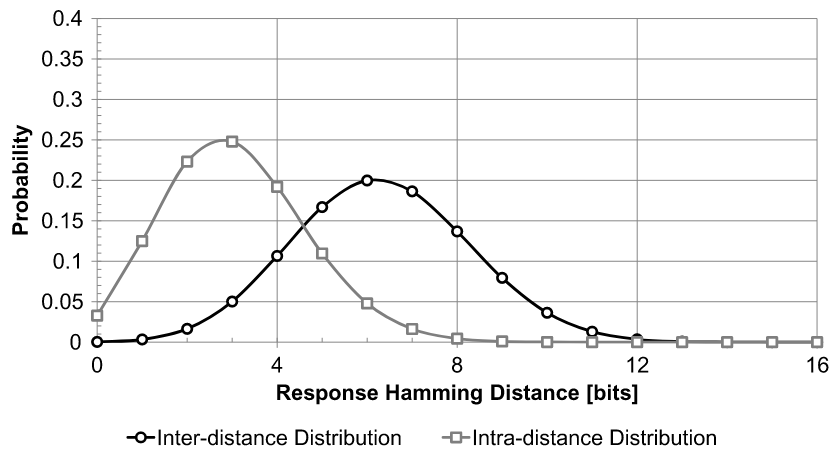
\includegraphics[width=0.7\textwidth]{inter-_intra-distance_distributions.png}
    \\
    Source: \cite[][p. 122]{Maes2013}
\end{figure}

As the inter-distance is generally larger than the intra-distance, this PUF can be considered to be identifiable.
However, there are only two assumptions, that can be made with certainty:
\begin{enumerate}
    \item Two responses with $HD = 0$ definitely stem from the same entity.
    \item Two responses with $HD > 8$ definitely stem from different entities.
\end{enumerate}

For all other distances, it is not certain wether the two responses stem from the same or different entities,
because the probability curves overlap. If there exists an overlap like this for a given PUF class,
a threshold distance $t_{id}$ needs to be defined, if it is to be used for identification.
All response pairs with a $HD$ below $t_{id}$ are considered to stem from the same instance.
All response pairs with a $HD$ above $t_{id}$ are considered to stem from different instances. \cite[][p. 121f]{Maes2013}

When identifying an entity, a CRP established during the enrollment phase is used and the response
generated during enrollment is compared to the response generated during identification.
This comparison can yield four different outcomes \cite[][p. 122f]{Maes2013}:
\begin{enumerate}
    \item \emph{True Acceptance}: The entity is the same one that was enrolled and $HD$ of both responses
          lies below $t_{id}$. The entity is correctly identified and accepted.
    \item \emph{False Acceptance}: The entity is different from the one that was enrolled and $HD$ of
          both responses lies below $t_{id}$. The entity is incorrectly identified and
          accepted.
    \item \emph{True Rejection}: The entity is different from the one that was enrolled and $HD$ of the
          responses lies above $t_{id}$. The entity is correctly rejected.
    \item \emph{False Rejection}: The entity is the same one that was enrolled, but the $HD$ of both responses
          lies above $t_{id}$. The entity is incorrectly rejected.
\end{enumerate}

The \ac{FRR} is the probability, that a given identification attempt will be falsely rejected.
It is simultaneously the probability, that the inter-distance is smaller than the identification threshold.
The \ac{FAR} is the probability, that a given identification attempt will be falsely accepted.
It is also the probability, that the intra-distance is larger than the threshold.
These metrics can be used to find the ideal threshold for the identification system \cite[][p. 123]{Maes2013}.
Figure \ref{fig:relationship_far_frr} shows the relationship between FRR and FAR for different PUF implementations.
The curves for each type show the FRR as a function of FAR.
If the threshold is lowered, the system will become more secure as the FAR decreases and the FFR increases.
If the threshold is increased (higher values for $HD$ are accepted), the system becomes more robust at the
cost of security.

\begin{figure}[H]
    \centering
    \caption{Relationship between FAR and FRR for different PUF implementations}
    \label{fig:relationship_far_frr}
    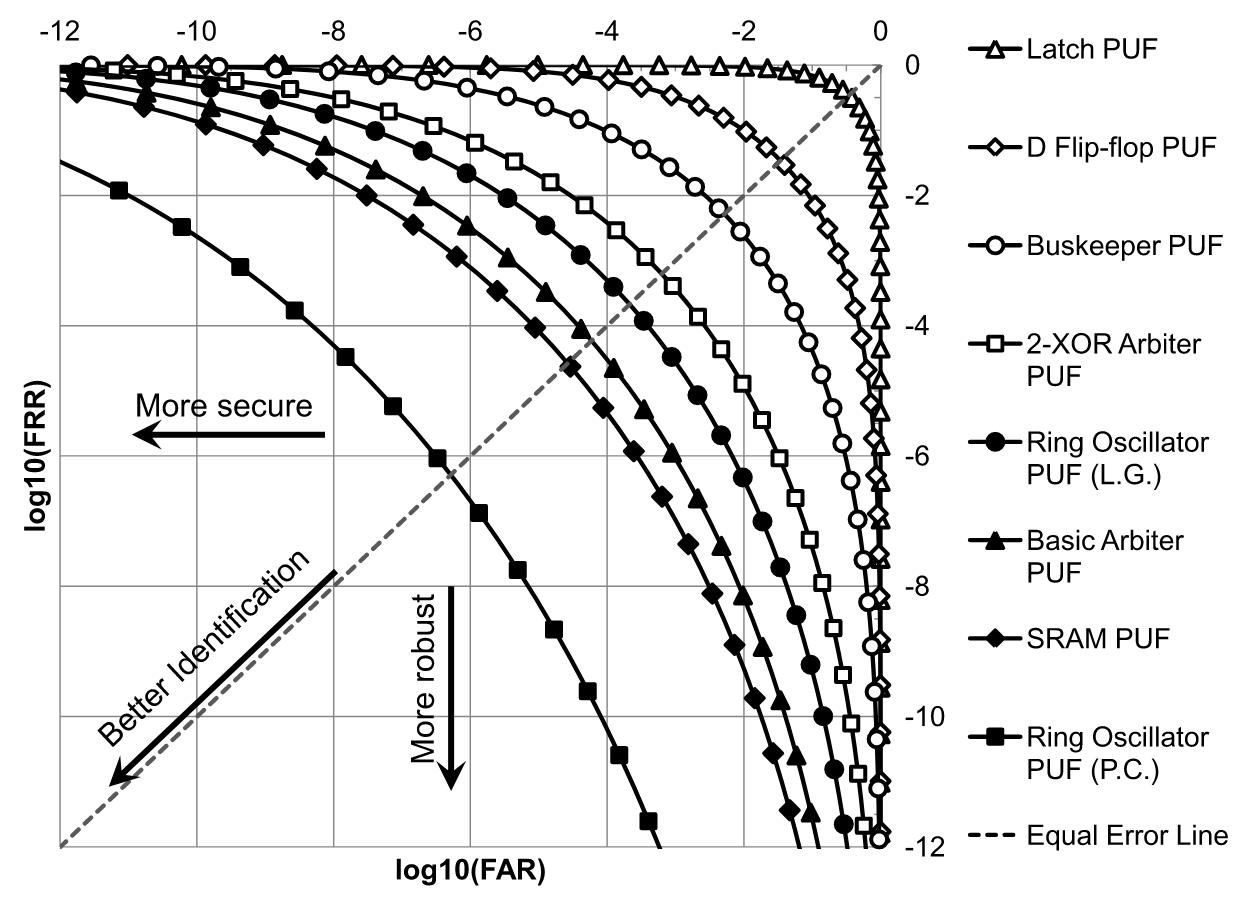
\includegraphics[width=0.7\textwidth]{relationship_far_frr.png}
    \\
    Source: \cite[][p. 125]{Maes2013}
\end{figure}

\subsubsection{Basic PUF-based Challenge-Response Authentication Protocol}
\label{sec:basic_challenge_response_protocol}

Challenge-Response protocols allow the inherent identifying features of PUFs to be used for authentication.
The most basic protocol used for PUF-based authentication is described here.

Like with identification, a challenge-response protocol using PUFs typically consists of two phases.
The first phase is \emph{enrollment}, which is identical to the first phase present in identification and
involves the verifier recording the identity of every entity by collecting many different \acp{CRP} from each
PUF and storing them in a database \cite[][p. 129f]{Maes2013}.
The verifier also assigns a unique ID to each entity and provides the entity with their ID.

\begin{figure}[h]
    \centering
    \captionsetup{justification=centering}
    \caption{UML Sequence Diagram showing the Enrollment Phase in the Basic Protocol}
    \label{fig:seq_dia_basic_protocol_enrollment}
    \begin{subfigure}{0.8\textwidth}
        \begin{plantuml}
            @startuml
            database DB as db
            participant Verifier as v
            collections "P Provers" as p
            group Enrollment Phase [for p in P where P is the number of provers]
            p -> v : Request Enrollment
            v --> p : OK
            v -> db : Create entity p
            db --> v : Entity ID for p
            loop for c in C where C is the number of CRPs
            v -> p : Send Challenge c
            p -> v : Send Response c
            v -> db : Store CRP c for ID
            db --> v : Success
            end
            v -> p : Send ID
            p --> v : OK
            end
            @enduml
        \end{plantuml}
    \end{subfigure}
    \\
    Source: Own design based on protocol proposed in \cite[][p. 129f]{Maes2013}
\end{figure}

The second phase is \emph{verification}, shown in figure \ref{fig:seq_dia_basic_protocol_verify}.
Here the authenticating entity first provides their unique ID.
The verifier looks up the available \acp{CRP} for that ID in the database and randomly selects one of them.
The respective challenge is then sent to the prover, which uses it to generate the response and sends it to
the verifier. The verifier then calculates the distance between the response recorded at enrollment
and the response received from the entity and checks, wether it is below a
previously defined authentication threshold $t_{auth}$.
If this check is successful, the entity is authenticated. The used CRP is then deleted from the database, so it
can not be used again. This protects against man-in-the-middle replay attacks \cite[][p. 130]{Maes2013}.
As previously described, there is room for error in this process, depending on how high or low $t_{auth}$ is set.

\begin{figure}[h]
    \centering
    \caption{UML Sequence Diagram showing the Verification Phase in the Basic Protocol}
    \label{fig:seq_dia_basic_protocol_verify}
    \begin{subfigure}{0.8\textwidth}
        \begin{plantuml}
            @startuml
            database DB as db
            participant Verifier as v
            entity "prover" as p
            group Verification Phase
            p -> v : Authentication Request with ID
            v --> p : OK
            v -> db : Request random CRP c
            db --> v : Send CRP c
            v -> p : Send challenge c
            p -> p : p.Eval(c)
            p -> v : Send response
            v -> v : Verify response
            alt accepted
            v -> p : Accepted
            else rejected
            v -> p : Rejected
            end
            end
            @enduml
        \end{plantuml}
    \end{subfigure}
    \\
    Source: Own design based on protocol proposed in \cite[][p. 129f]{Maes2013}
\end{figure}

\subsection{Other Applications for PUFs}
\label{sec:puf_applications}

In addition to authentication, PUFs can also be applied different scenarios.
The following is a short overview of alternative use-cases for PUFs, to get a sense of their
versatility.

\subsubsection{Storage and Generation of Cryptographic Keys}

As explained in section \ref{sec:strong_weak_pufs}, weak PUFs are not ideal for authentication, but have different uses.
One application for weak PUFs is to generate and store cryptographic keys.
The security of cryptographic protocols is entirely reliant on selecting a key with appropriate entropy
and keeping that key secret.
If an attacker were to extract the key from memory, application code or a database, the security of the given
system is compromised. \cite[][p. 3f]{McGrath2019}

By using PUFs, keys don't have to be stored permanently, but can instead be generated on demand by the PUF,
stored temporarily in memory and deleted after usage.
Essentially, the PUF itself acts as a key that only generates a copy, which is kept for a short period of time.
A challenge is sent to the PUF to generate a key (response) from it.
The response is never entirely precise, so error correction is used to ensure that keys are consistent.
Next, the response is converted into a uniform key using a hash function, which can then be used for encryption. \cite[][p. 884f]{Katzenbeisser2012}

Even though weak PUFs don't have a large set of \acp{CRP}, the central properties of PUFs are still essential.
The PUF needs to be unpredictable, so an attacker is not able to create a model
of the PUF used for key generation. If the attacker were able to do this, they could generate the appropriate
key and intercept communications.
The PUF also needs to be unclonable, so no third-party is able to have direct access to the exact \acp{CRP}.
It needs to be robust, so the same key is always generated for a given challenge. \cite[][p. 885]{Katzenbeisser2012}

\subsubsection{Object Identification}

This is again a good use-case for weak PUFs, as the burden of proving the identity is eliminated,
allowing the use of less secure constructions.
In terms of weak PUFs, identification of specific instances of a class could again be done by using a single \ac{CRP}.
After manufacturing, a generic challenge could be posed to each instance and responses could be recorded in a database.
If the identity of a device is to be established at a later point, one would simply have to issue the same challenge
to the instance and look up the response in the database \cite[][p. 118]{Maes2013}.
An example use-case for object identification would be tracking specific products in a logistics system \cite[][p. 118]{Maes2013}.
One could also use this method to detect counterfeit products, as the counterfeit would not be able to have the same
response behavior as the original, because PUFs are unclonable \cite[][p. 884]{Katzenbeisser2012}.

\subsubsection{Internet of Things}

The two applications explained above both deliver great value in the \ac{IoT} space.
As more devices and appliances in the daily life of consumers become connected and "smart",
there is a need to create trust in these devices and ensure security.
By having IoT devices generate the keys they use to authenticate to external systems using
intrinsic random variations, their identity can be reliably and consistently verified.
Constructions like the \ac{SRAM} PUF are especially interesting in this regard, as they do not require modifications
to hardware and can be applied to all classes of existing electronic devices that use embedded SRAM
memory. \cite[][p. 88]{Gao2020}
\newpage
\section{Prototype Implementation of a Protocol}
\label{sec:implementation}

\subsection{Selecting a Protocol}
\label{sec:imp_selection}

The initial plan for this thesis was to take the knowledge gained from the literature review
and use it to design a new protocol, which combines the best features of each
protocol to perfectly fit the requirements of the research project.
However, during the review it became clear, that the design of such a protocol is far
out of scope for this thesis, as extensive knowledge of cryptography and extensive
security proofs are needed to ensure the security of the protocol.
Due to this fact, the methodology is changed and one of the reviewed protocols is selected,
based on the requirements.
The protocol is then examined closely in order to fully understand it.
After that, a prototype of the infrastructure is implemented.

The goal of the research project, that this thesis is a part of, is to design a complete
authentication system, that can be used in an electronic locking system for physical access protection.
There are several criteria that can be derived from this goal:
\begin{itemize}
    \item To prevent unauthorized persons from entering protected areas, security is of the highest importance.
          The protocol should thus not be susceptible to any known attacks that could compromise the integrity of the system.
    \item The system should be practical for daily use when entering buildings, floors or rooms.
          Therefore, authentication needs to be fast, and there needs to be an easy and secure way for
          the authentication device to interface with the system.
    \item Authentication needs to be possible at multiple physical entry points
    \item Privacy and anonymity are important, because users would carry these devices
          with them for long periods of time, potentially allowing attackers to track them.
\end{itemize}

Looking at the reviewed papers in table \ref{tbl:review_results}, \cite{Gope2018}, \cite{Zhu2019} and \cite{Hristea2019} immediately
seem like good choices, because they are focused on the use-case of RFID.
This would allow the PUF devices to be embedded in RFID tags, which could interface with RFID readers
at every required physical entry point to authenticate persons against the system and grant access.
In addition, \cite{Zhu2019} delivers solid proofs for all security related features,
does not require any special PUF implementation, is able to handle noisy PUF responses
and is proven to be scalable. Therefore, this protocol is selected.

In the next section, the protocol is thoroughly examined.

\subsection{Design of the Protocol}
\label{sec:imp_design}

\subsubsection{Assumptions}

Two versions of the protocol were proposed by \citeauthor*{Zhu2019}. One version assumes an ideal PUF with
intra-distance $HD = 0$, while the other uses fuzzy extractors to deal with
noise in PUF responses \cite[][p. 6, 8]{Zhu2019}.
To keep the complexity manageable for the implementation phase, the simplified version of the protocol
is examined in this thesis. This means, that from now on, the PUF is considered to have ideal challenge-response
characteristics.
In a future work, this could easily be improved upon by implementing the enhanced version of the protocol,
which is specified in great detail in the paper \cite[][p. 8]{Zhu2019}.

Figure \ref{fig:protocol_structure} shows the layout of the underlying RFID system, including the three parties
backend server, reader and tag. The tag is a small device embedded with a PUF module, which has inherently unique
characteristics. The backend server and reader are connected through a secure channel, which an attacker
does not have access to. A physical attack on the tag is assumed to change the behavior of the PUF and make
the tag useless. Both tag and server have access to a hash function, which generates the same output for a given
input on both sides. The tag is considered to be resource limited, which means that the protocol does not specify any
spatially or computationally intensive tasks on the tag \cite[][p. 5]{Zhu2019}.

\begin{figure}[H]
    \centering
    \caption{Layout of the RFID infrastructure}
    \label{fig:protocol_structure}
    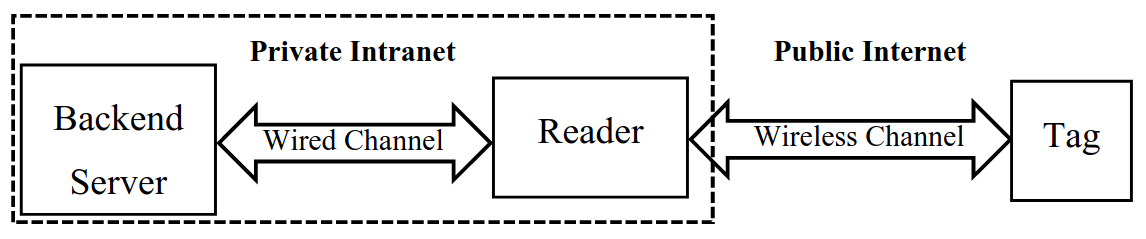
\includegraphics[width=0.7\textwidth]{structure_of_protocol.png}
    \\
    Source: \cite[][p. 5]{Zhu2019}
\end{figure}

In addition to the hash function, each party requires two more operations.
One is an XOR operation, denoted as $\oplus$, the other is a concatenation of two bitstrings, denoted as $\parallel$.

The protocol consists of two phases, the setup phase and the authentication phase. \cite[][p. 6-8]{Zhu2019}

\subsubsection{Setup Phase}

The setup phase only needs to be executed once in the beginning to initially synchronize tag and server over a
secure channel. It is comparable to the enrollment phase discussed for the basic protocol in section \ref{sec:basic_challenge_response_protocol}.
After that, the authentication phase can happen over an insecure channel \cite[][p. 7]{Zhu2019}.
Figure \ref{fig:protocol_setup} shows a sequence diagram of the setup phase.

\begin{figure}[H]
    \centering
    \caption{Setup Phase of the Proposed Protocol}
    \label{fig:protocol_setup}
    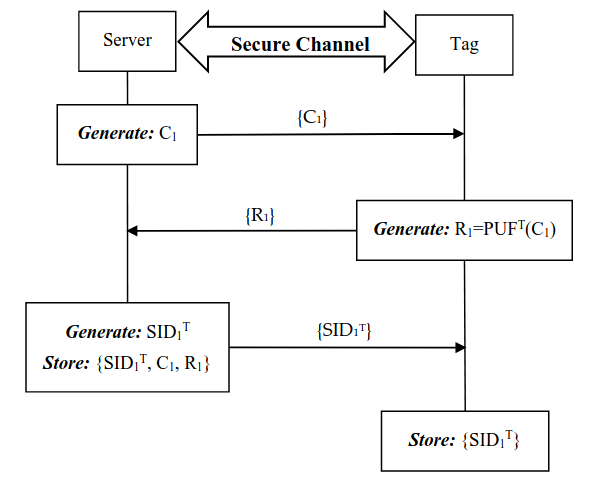
\includegraphics[width=0.7\textwidth]{setup_phase.png}
    \\
    Source: \cite[][p. 6]{Zhu2019}
\end{figure}

In the first step, the server generates a challenge and sends it to the tag.
The tag evaluates its internal PUF module using the challenge, producing a response.
The response is sent back to the server.
Next, the server prepares a unique session identity $SID$, which is used later in the first round of
authentication. The server sends it to the tag, which stores it in memory.
The server stores the $SID$, as well as the \ac{CRP} for the tag.
This concludes the setup phase. The tag is now enrolled in the system an can be used for authentication
from now on. \cite[][p. 7]{Zhu2019}

This process can be repeated for an arbitrary number of tags. The server generates a different challenge
and $SID$ for each tag and stores all of them in its database. \cite[][p. 7]{Zhu2019}

\subsubsection{Authentication Phase}

The authentication phase is described next.
Note that the reader is not shown in figure \ref{fig:protocol_authentication}, as it is connected with the server through a
secure channel. Therefore, server and reader are seen as a single unit. In reality, the messages from
the tag would be received by the reader and then forwarded to the server.
Figure \ref{fig:protocol_authentication} shows the $i$-th round of authentication.
This means that variables like $C_i$ and $R_i$ are used in the current round of authentication,
while variables like $C_{i+1}$ are prepared for the next round.

\begin{figure}[H]
    \centering
    \caption{Authentication phase of the proposed protocol}
    \label{fig:protocol_authentication}
    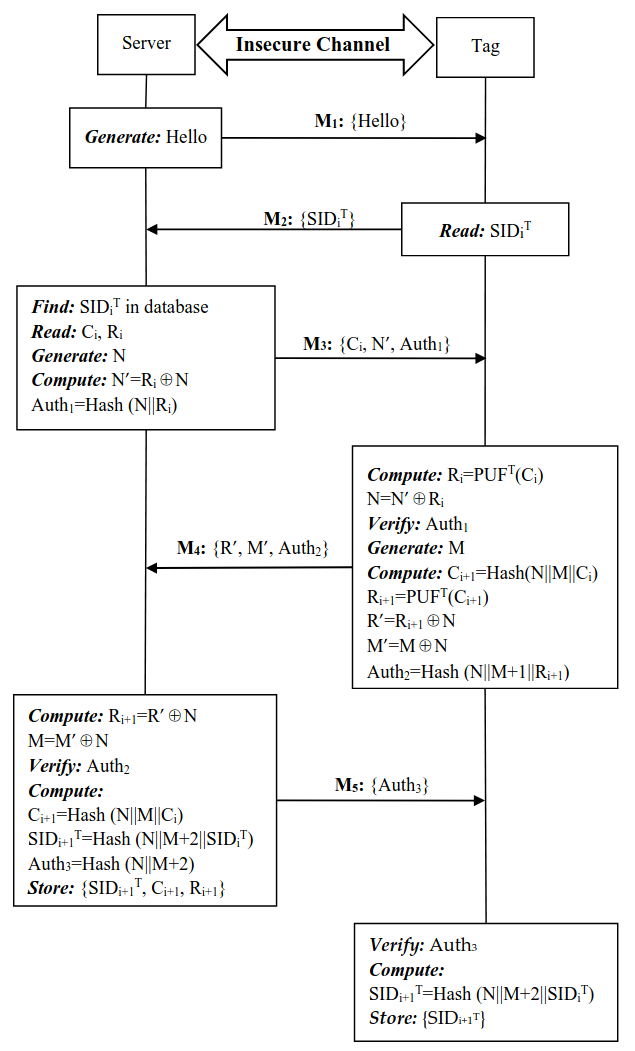
\includegraphics[width=0.7\textwidth]{authentication_phase.png}
    \\
    Source: \cite[][p. 7]{Zhu2019}
\end{figure}

In the first step, the server sends a "Hello" message to initiate the protocol. The tag answers this
with the session identifier it received during the setup phase or a previous authentication phase. \cite[][p. 7]{Zhu2019}

Next, the server uses the $SID$ to find the previously stored \ac{CRP} for that tag in the database.
If it can't find the $SID$ in the database, the tag is considered to be invalid and the authentication phase is
terminated.
Next it generates a random number $N$ and performs an XOR operation $R_i \oplus N$ on the random number and the response
to produce $N'$. It hashes a concatenation of $N$ and the response to produce $Auth_1$.
The challenge, $N'$ and $Auth_1$ are sent to the tag. \cite[][p. 7]{Zhu2019}

The tag uses the challenge $C_i$ sent by the server to evaluate its PUF module and produce
the response $R_i$. Note that in this scenario, the PUF is considered ideal, so the response is equal to the one the
server had stored in its database.
It uses the response and $N'$ to perform the same XOR operation and compute $N$.
It then produces the same hash from $N$ and the response as the server to verify $Auth_1$, as proof that
the server is genuine, because knowledge of $R_i$ is needed to calculate $Auth_1$ in the first place.
After verification, it generates a second random number $M$ and uses it to compute the next challenge $C_{i+1}$
which is a hash of the concatenation of $N$, $M$ and the challenge $C_{i+1}=Hash(N\parallel M \parallel C_i)$.
The PUF is evaluated using $C_{i+1}$ to produce the next response $R_{i+1}$.
$R'=R_{i+1} \oplus N$ and $M' = M \oplus N$ are calculated using XOR operations on $N$.
Lastly, the tag calculates $Auth_2 = Hash(N \parallel M+1 \parallel R_{i+1})$.
It sends $R'$, $M'$ and $Auth_2$ back to the server. \cite[][p. 7]{Zhu2019}

The server uses $R'$ and $M'$ received from the tag to compute $R_{i+1}$ and $M$ in the same way as the tag.
It uses them to verify $Auth_2$, which proves the identity of the tag, as the tag would not be able to generate
a correct $Auth_2$ without knowing $N$, which requires knowledge of the response to $C_i$,
that it can only know using the PUF module.
It computes the next challenge $C_{i+1}$, the next session identity $SID_{i+1}$ and $Auth_3$.
The server stores the next sid, and the next \ac{CRP} in its database and sends $Auth_3$ to the tag.
However, the old CRP and $SID$ are still kept in the database, to prevent desynchronization attacks.
The tag verifies $Auth_3$ in the same way, computes the next session ID and updates it internally. \cite[][p. 7]{Zhu2019}

If during this process, verification of any of the three $Auth$ parameters fails on either party,
the authentication procedure should be terminated to prevent attacks. If all validations pass,
each party has proven their identity to the other party. They are thus mutually authenticated. \cite[][p. 7]{Zhu2019}

\subsection{Python Implementation}
\label{sec:imp_solution}

A basic prototype of the protocol was implemented using Python.
Note that the full code is not shown in the text to improve readability and focus
on the important details. For the full implementation, refer to \ref{sec:appendix_code}.

\subsubsection{Simulating the PUF Module}

The PUF module was simulated using the \emph{pypuf} Python library \cite{pypuf}.
It provides simulations for many of the major strong PUFs, including Arbiter PUFs and Optical PUFs.
For this implementation, the \emph{ArbiterPUF} simulation was used.
The following code shows how the simulation is used in code:
\begin{lstlisting}[language=Python]
>>> from pypuf.simulation import ArbiterPUF
>>> puf = ArbiterPUF(n=64, seed=1)
>>> from pypuf.io import random_inputs
>>> puf.eval(random_inputs(n=64, N=3, seed=2))
array([ 1,  1, -1], dtype=int8)
\end{lstlisting}

The constructor takes the number of switch gates, which equals the number of challenge bits, and a seed
which defines the random characteristics of the PUF module.
The library additionally supports setting a level of noisyness for the PUF, however this was not used here.
The PUF instance provides a $puf.eval()$ method, which takes a two dimensional array of shape $(N, n)$,
where $n$ is the number of challenge bits and $N$ is the number of evaluations.
Each value of the array is an integer  of either $-1$ or $1$, which dictates wether that switch is turned on or off.
The PUF returns an array of length $N$, because on each evaluation of the PUF, a single value is returned.
The response consists of the results of $N$ evaluations, making it length $N$.

While testing, it was noticed that for small $N$, it is easy to have colliding PUF responses for different challenges,
which would decrease security of the implementation.
In the end, $N = 8; n = 64$ was used, as it proved to have no problems with value collisions, even at a high
number of evaluations.

\subsubsection{Additional Dependencies}

For hashing, the \emph{sha256} hash function from the builtin Python \emph{hashlib} was used.
The library provides a number of hash functions, which can easily be imported and used to hash different types of data.
There is no particular reasoning behind the choice of \emph{sha256} for hashing. As there are no hardware constraints
for this implementation, complexity was not an issue. However on a real RFID tag, one would not be able
to implement \emph{sha256}, as the number of logic gates required is far too high.
Therefore, in a real-world setting, a different lightweight hash function, like \emph{SPONGENT}, should be used \cite[][p. 2]{Zhu2019}.

To represent the binary challenges and responses, the Python \emph{bitstring} library was used.
It provides a \emph{BitArray} class, which allows storing binary data in a space efficient way, while also
providing methods to convert hex or integer data to binary and vice-versa, which proved useful during the
implementation of the protocol steps.
The \emph{numpy} library was used to convert the PUF responses from the \emph{ArbiterPUF} modules to and from \emph{BitArrays}.

For the creation of $SID$s, a source of randomness was needed. For this, the Python builtin \emph{uuid} module,
as well as the \emph{random} module were used.

The \emph{pytest} framework was used for testing the implementation.

\subsubsection{Structure of the Program}

The structure of the main program is shown in figure \ref{fig:implementation_structure_main}.
It consists of four main classes \emph{Server}, \emph{Tag}, \emph{TagFactory} and \emph{AuthSession}.

\begin{figure}[H]
    \centering
    \caption{UML Class Diagram showing Structure of Main Implementation}
    \label{fig:implementation_structure_main}
    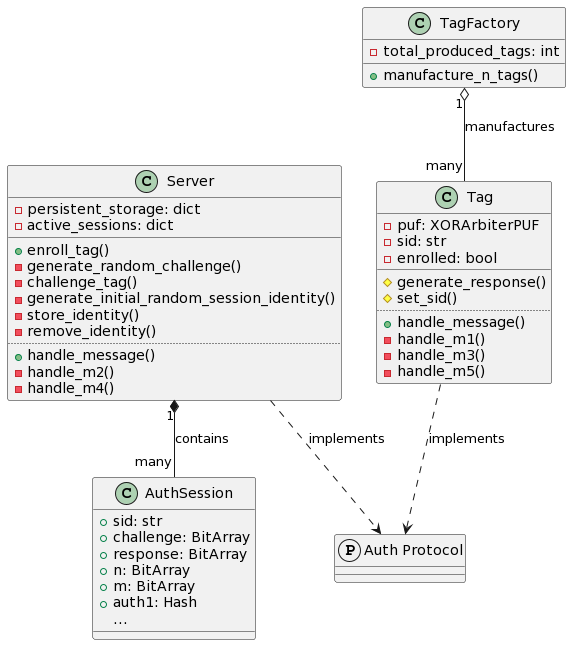
\includegraphics[width=0.7\textwidth]{implementation_structure_main.png}
\end{figure}

\emph{Server} and \emph{TagFactory} are implemented using a singleton pattern to ensure, that only one instance
can be present at all times, which helps to keep state consistent.
\emph{TagFactory} keeps track of the number of total produced \emph{Tags}, which is important for managing random variations.
As the \emph{ArbiterPUF} takes a seed integer, the factory needs to ensure, that no two tags with the same
seed are created, as they would have PUF modules with the same characteristics.
Therefore, each produced tag is assigned a different seed based on the total number of tags in existence.

The server has two types of storage, a dictionary storing active sessions of type \emph{AuthSession} and
a persistent storage dictionary, which is used for storing $SID$s and CPRs for all enrolled tags.
The server also provides an \emph{enroll\_tag} method, which takes a tag and a challenge seed and
executes the setup phase of the protocol with the tag, so it can be used for authentication in the future.
\emph{AuthSession} is a type responsible for storing all relevant data needed in the authentication phase.
The server supports the use of multiple readers at the same time, which allows multiple \emph{Tags} to be
authenticated simultaneously. Each active authentication phase needs its own \emph{AuthSession}.
The sessions are destroyed, once the tag has been authenticated and the new $SID$ and CRP have been stored
in persistent storage.

A \emph{Tag} consists of a PUF module, a variable for storing the $SID$ and a boolean which keeps track of
whether the tag has been enrolled by the server.
It also has two methods for generating responses and setting the $SID$ on the tag, which the server can call directly
during the setup phase.

Both \emph{Tag} and \emph{Server} provide a \emph{handle\_message} method.
It is used for communication between the two entities during the authentication phase.
The server \emph{handle\_message} takes an \emph{AuthMessage} , and a reader ID, which is needed to keep track of the different
simultaneous \emph{AuthSessions}. The tag's \emph{handle\_message} only takes messages, as it does not need to
keep track of sessions.

Server and Tag both implement the Auth Protocol, but this is only included in the class diagram for the purpose of
showing that both entities support the protocol. There is no specific \emph{AuthProtocol} type implemented.

In addition to the main entities described above, there is an external \emph{support} module which provides
all necessary supporting functions and constants, that are not defined by the protocol, but both parties need
to agree on.
The support module structure is shown in figure \ref{fig:implementation_structure_support}.
It includes constant values for the length of challenges and responses, as well as the hash function that
should be used by each party to verify responses.
It also provides functions for converting numpy arrays to \emph{BitArrays}, as the PUF module takes and returns
numpy arrays, but the rest of the program uses \emph{BitArrays} for handling binary data, as they
have better compatibility with hash functions and other calculations.
The basic operations required by the protocol are also provided, including creation of
a new hash, verifying a hash, XOR and concat, among others.

\begin{figure}[H]
    \centering
    \caption{UML Class Diagram of the Support Module}
    \label{fig:implementation_structure_support}
    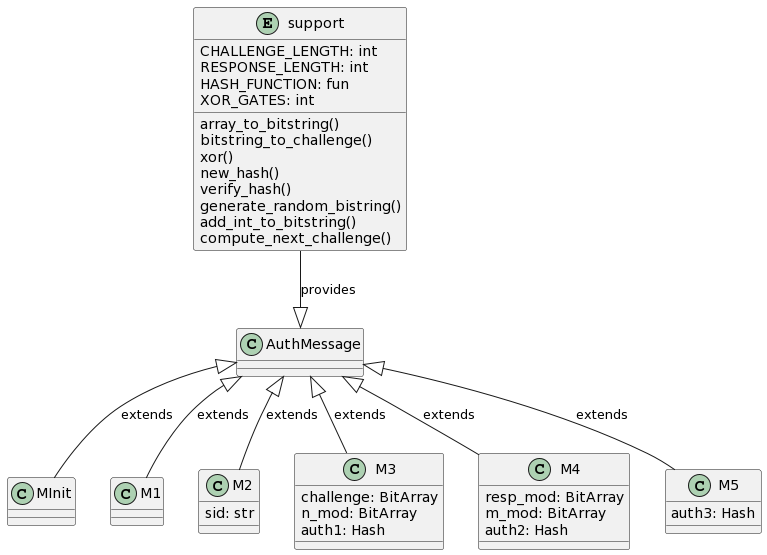
\includegraphics[width=0.8\textwidth]{implementation_structure_support.png}
\end{figure}

Lastly the \emph{support} module provides types for each of the messages required for the authentication phase.
These classes extend a common class \emph{AuthMessage} and each message holds different values, like \emph{sid}, \emph{challenge},
or \emph{auth} values, depending on what data is being sent in that step of the authentication phase.
The \emph{handle\_message} endpoint of both tag and server takes the \emph{AuthMessage} type and all of its children
and uses the specific type internally, to ensure that communication is synchronized and that
each message is handled according to protocol.

\subsubsection{Enrollment of Tags}

The following code sets up the infrastructure,
manufactures $n = 10$ tags with unique PUF modules and enrolls them with the server:

\begin{lstlisting}
factory = TagFactory()
server = Server()
n = 10
tags = factory.manufacture_n_tags(10)
for seed, tag in enumerate(tags):
    server.enroll_tag(tag, seed)
\end{lstlisting}

First, the factory and server are instantiated.
Next the factory's manufacturing method is called with the number of tags that should be created.

The code for tag creation looks like this:

\begin{lstlisting}
def manufacture_n_tags(self, n) -> List['Tag']:
    tags = []
    for i in range(0, n):
        seed = self.total_produced_tags
        puf = ArbiterPUF(n=CHALLENGE_LENGTH, seed=seed)
        tags.append(Tag(puf))
        print(f"Tag with seed {seed} manufactured")
        self.total_produced_tags += 1

    return tags
\end{lstlisting}

The seed for the PUF module is directly taken from the factories total production count.
This makes sure that each tag has a unique challenge response behavior. It also makes the behavior
of tags very predictable, but this can be ignored, because in the real world the behavior
would stem from uncontrollable intrinsic variations.
The PUF is created with the challenge length provided by the support module.
A new tag object is instantiated with the PUF module and added to the list of tags.
The list is then returned, concluding the production process.

Next, the newly created tags need to be enrolled.
Therefore, the server's enroll\_tag method is called directly for each tag.
The following code shows that method:

\begin{lstlisting}
def enroll_tag(self, tag: tag.Tag, challenge_seed: int) -> None:
    challenge = self.generate_random_challenge(challenge_seed)
    response = self.challenge_tag(tag, challenge)
    sid = self.generate_initial_random_session_identity()
    self.store_identity(sid, challenge, response)
    tag.set_sid(sid)
    print("Enrolled Tag with SID ", sid)
\end{lstlisting}

It takes the tag and a challenge seed, which it uses to generate a random challenge of the correct length.
It then calls the server's challenge\_tag method, which triggers the tag's PUF module to generate a response.
Next, a session id is generated and SID and the CRP are stored in the server's persistent storage.
Lastly, the SID is set in the tag's memory and the enrollment is finished.

\subsubsection{Authentication Phase}

To demonstrate the authentication phase, the mutual authentication of a single tag is shown here.
We assume a fully set up infrastructure with Tag \emph{tag} and Server \emph{server}.
The following code executes the authentication phase and returns a success message:

\begin{lstlisting}
tag = tags[0]
reader = 0
m1 = server.handle_message(support.MInit(), reader)
m2 = tag.handle_message(m1)
m3 = server.handle_message(m2, reader)
m4 = tag.handle_message(m3)
m5 = server.handle_message(m4, reader)
success = tag.handle_m5(m5)
if success:
    print("Tag with SID: ", tag.sid, "successfully mutually authenticated.") 
\end{lstlisting}

The server's and tag's handle\_message methods are called in an alternating way,
using the previous message returned by the other party as an argument each time.
Note that the server's method takes two arguments, to account for the use of multiple
RFID readers at the same time on a single server.
The next piece of code shows the server's handle\_message method:

\begin{lstlisting}
def handle_message(self, m: AuthMessage, reader_id: int) -> None:
    if reader_id in self.active_sessions:
        session = self.active_sessions[reader_id]
    else:
        session = self.AuthSession()
        self.active_sessions[reader_id] = session
        session.expected_message = MInit
    if type(m) != session.expected_message:
        raise TypeError(
            f"Expected {session.expected_message}, got {type(m)}")
    elif (type(m)) == MInit:
        session.expected_message = M2
        return M1()
    elif (type(m)) == M2:
        session.expected_message = M4
        return self.handle_m2(m, session)
    elif (type(m)) == M4:
        m = self.handle_m4(m, session)
        del self.active_sessions[reader_id]
    
        print(f"Tag at reader {reader_id} successfully authenticated.")
        print("New session identity written to persistent storage\n")
        return m
    else:
        raise TypeError("Unknown Message Type")

\end{lstlisting}

It first checks if there is an active session for the given reader and creates a new one if there is none.
Next it checks which type of message was sent and calls the appropriate internal method to handle
that message. To ensure consistency within a session, the last received message is recorded and
an expected\_message variable is set, which is checked before each handling call.
After handling M4, the session is deleted from the session memory, as the tag is now successfully authenticated.

The code of handle\_m2 is shown next to explain handling of specific messages:

\begin{lstlisting}
def handle_m2(self, m, session: AuthSession) -> M3:
    session.sid = m.sid
    try:
        session.challenge = self.persistent_storage[session.sid]["c"]
        session.response = self.persistent_storage[session.sid]["r"]
    except KeyError:
        raise ValueError(
            "Invalid SID sent by tag.\nTag might be invalid. Authentication terminated.")

    session.n = generate_random_bitstring(RESPONSE_LENGTH)
    session.n_mod = xor(session.response, session.n)
    session.auth1 = new_hash(
        bytes(concat(session.n, session.response).hex, 'utf-8'))
    return M3(session.challenge, session.n_mod, session.auth1)
\end{lstlisting}

M2 is sent by the tag after the initial hello message and contains the SID stored in the tag's memory.
It is stored in the session, then the persistent\_storage of the server is queried, to find the
CRP stored during enrollment or a previous authentication phase. If it is not found, the tag is assumed to
be invalid and needs to be re-enrolled.
The session generates $N$ not as an integer, but in the form of a random BitArray of length \emph{RESPONSE\_LENGTH}.
This is done so it is possible to easily perform XOR operations on the random number with the challenge.
\emph{n\_mod} represents $N'$ from the protocol definition.
\emph{auth1} is created by hashing the hexadecimal representation of the concatenation of $n$ and the $response$.
$n$, $n\_mod$ and \emph{auth1} are all stored in the session and returned in \emph{M3}.

Only a small part of this implementation has been shown in this section. To look at the full code, please reference
\ref{sec:appendix_code}.

\subsubsection{Testing the Implementation}

To test the implementation, some rudimentary test scenarios were developed using the \emph{pytest} framework.
It provides methods for asserting, wether a variable has taken on the correct value, or
if the correct errors were raised during execution.
The following tests were implemented:
\begin{itemize}
    \item Enrolling 100 tags and authenticating them in sequence.
    \item Enrolling 100 tags and authenticating them in parallel, using 100 different readers.
    \item Enrolling a single tag and authenticating it 100 times in sequence,
          to test if generation of new CRPs and SIDs works correctly.
    \item Enrolling two tags and switching them in the middle of the authentication process
          on the same reader. This should raise a ValueError, as the hashes should not be able
          to be verified.
    \item Enrolling a tag and changing its SID before the authentication phase.
          This should again lead to a ValueError, as the SID should not be found in the server's
          database.
    \item Enrolling a tag and modifying its internal PUF module before authentication.
          This would be the equivalent of an attacker tampering with the tag and changing
          the PUFs characteristics. This should raise a ValueError, as the challenge response
          behavior has changed.
\end{itemize}

As an example the last test is shown here:

\begin{lstlisting}
def test_tag_with_invalid_puf():
    """An enrolled tag with a PUF module, that was modified by an attacker,
    should not be able to authenticate."""
    factory = TagFactory()
    server = Server()
    tag = factory.manufacture_n_tags(1)[0]
    server.enroll_tag(tag, 0)

    attacker_puf = ArbiterPUF(n=CHALLENGE_LENGTH, seed=1)
    tag.puf = attacker_puf

    m1 = server.handle_message(MInit(), 0)
    m2 = tag.handle_message(m1)
    m3 = server.handle_message(m2, 0)
    with pytest.raises(ValueError):
        tag.handle_message(m3)
\end{lstlisting}

After enrollment, the puf variable of the tag is reassigned to a newly created ArbiterPUF instance
with a different seed. Following this, a ValueError is raised, because the authentication hash
can not be verified on the tag's side.
This could still be circumvented by an attacker, by disabling the tag-side hash verification,
but the tag still would not be able to generate $Auth_2$ correctly, due to
the different PUF response.

Note, that these tests do not represent a comprehensive security analysis of the protocol, but give some sense
of its capabilities. For the complete set of tests, refer to \ref{sec:appendix_code}.